\documentclass{standalone}

\usepackage{tikz}
\usetikzlibrary{shapes,arrows}
\usetikzlibrary{calc}
%\usepackage{amsmath,bm,times}

\newcommand{\algoinput}[1]{\colorbox{yellow}{#1}}
\newcommand{\algooutput}[1]{\colorbox{orange}{#1}}

\graphicspath{
  {scripts/algo-calibration/} 
  {algo-calibration/}
}

\begin{document}

% We declare layers
\pgfdeclarelayer{background}
\pgfsetlayers{background,main}

% Define a few styles and constants
\tikzstyle{block}=[draw, text centered]
\tikzstyle{dim}=[text centered,node distance=1.5cm, scale=0.5,color=gray]

\def\m{5em}
\def\K{4em}
\def\B{6em}
\def\n{3em}

\begin{tikzpicture}[node distance=1.5cm]
  %%%%%%%%%%%%%%%%%%%%%%%%%%%%%%%%%%%%%%%%%
  %% STEP 1: SORTED PERMUTATION P-VALUES %%
  %%%%%%%%%%%%%%%%%%%%%%%%%%%%%%%%%%%%%%%%%
  % groups
  \node (groups) at (-1,0) {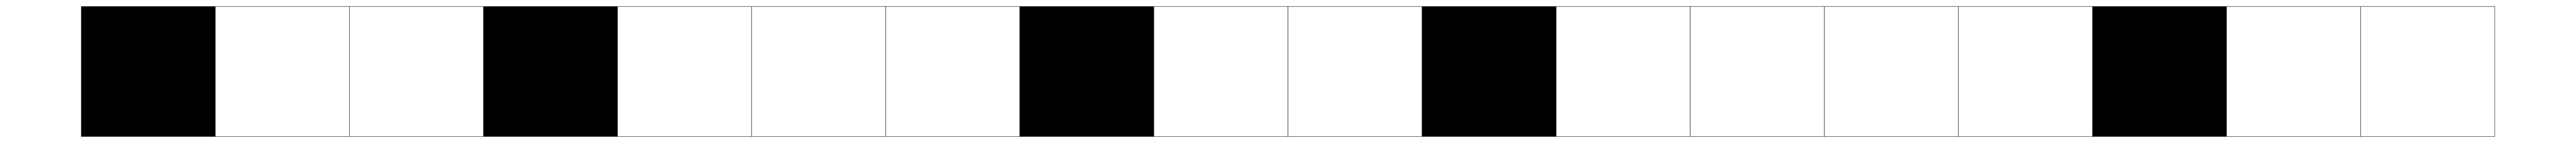
\includegraphics[width=1.5cm]{groups}};
  \node (groups-label) [above of=groups, node distance=1em] {\algoinput{group labels: $c$}};
  \node (1n) [dim, below of=groups, node distance=0.8em] {$1 \times n$};

  \node (groups perm) at (-1, -2.7) {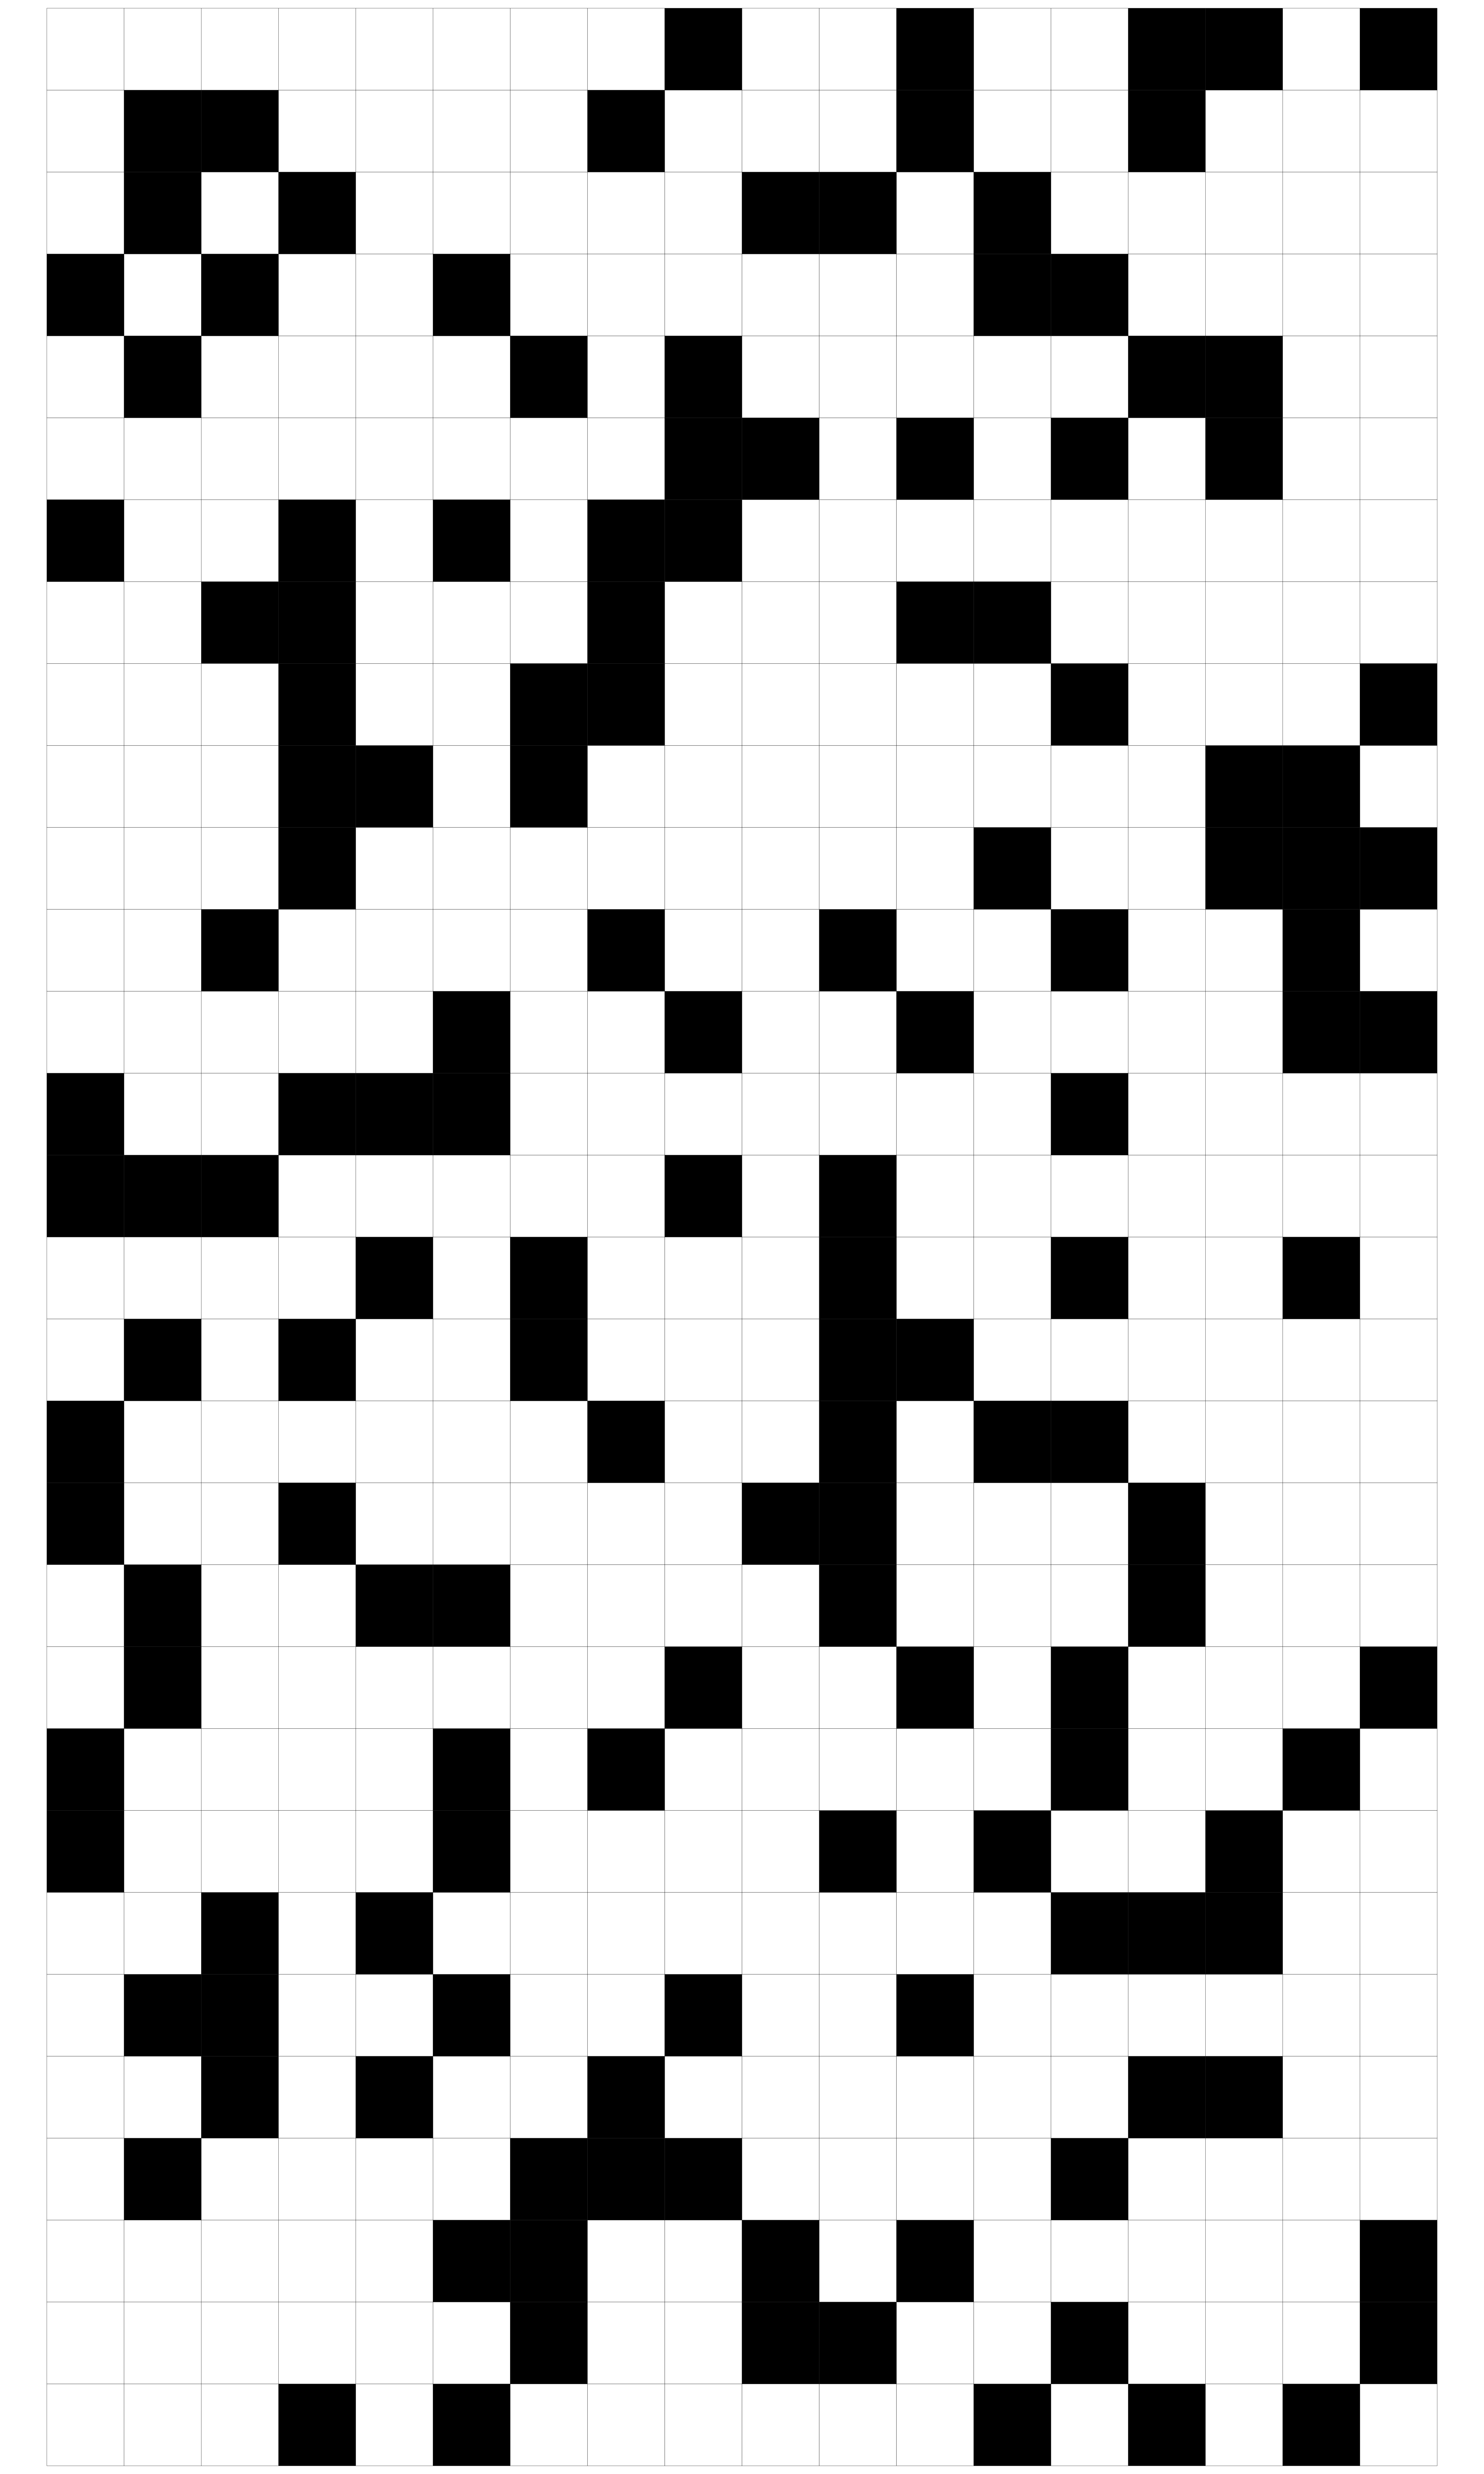
\includegraphics[width=1.4cm]{perm_groups}};
%  \node (B) at (-1.5, -1) {\algoinput{$B$}};
  \node (sample) at (-3, -1.5)[rotate=90] {\algoinput{$B$} permutations};
  \node (Bn) [dim, below of=groups perm, anchor=west, node distance=\B+1.5em] {$B \times n$};

  % X
  \node (data) [block, text height=\n, text width=\m, right of = groups, anchor=west, node distance = 2.3cm] {\algoinput{Data: $X$}}; % n*m
  \node (nm) [dim, below of=data, anchor=west, node distance=\n+1.4em] {$n \times m$};

  % test
%  \node (test) [right of = data, anchor=west] {\algoinput{$p$}};

  % p0
  \node (null p) [block, text height=\B, text width=\m, below of=data, anchor=north] {$P$}; % B*m
%   \node (null p in) [text height=\B, text width=\m, above = null p] {z}; % 
  \node (Bm) [dim, below of=null p, anchor=west, node distance=\B+1.5em] {$B \times m$};

  % sorted p0
  \node (sorted null p) [block, text height=\B, text width=\m, right of=null p, anchor=west, node distance=2.5cm] {$P_0$}; % n*1
  \node (Bm2) [dim, below of=sorted null p, anchor=west, node distance=\B+1.5em] {$B \times m$};

  \node (perm p title) [above of=data, anchor=north east] {\textbf{1. Permutation $p$-values}};

  % Arrows
  \draw[->] (data) -- (null p);
  \draw[->] (-1.8,0) to[out=180,in=180] (-1.8,-2.75);
  \draw[->] (-1.8,0) to[out=180,in=180] (-1.8,-2);
  \draw[->] (-1.8,0) to[out=180,in=180] (-1.8,-3.5);

  \draw[->] (-3,0) + (groups perm) -- node[above]{\algoinput{Test: $p$}} (null p);
  % \draw[->] (0.8,-2.75) to (1.2, -2.75);
  % \draw[->] (0.8,-2)    to (1.2, -2);
  % \draw[->] (0.8,-3.5) to (1.2, -3.5);

  % \draw[->] (test) -- (null p);
  \draw[->] (null p) -- node[above]{sort} (sorted null p);


  %%%%%%%%%%%%%%%%%%%%%%%%%%%%%%%%
  %% STEP 2: PIVOTAL STATISTICS %%
  %%%%%%%%%%%%%%%%%%%%%%%%%%%%%%%%
  % t_inv
%  \node (t_inv) [right of=sorted null p, anchor=west] {\algoinput{($\tau^{-1}_k)_{k=1\dots K}$}}; % B*K
%   \node (t inv) [block, text height= \B, text width=\K, below of=sorted null p, anchor=north west, node distance=3cm] {$t^{-1}(p(X_{\cdot (k:m)}^{(b)}))$}; % B*K
   \node (t inv) [block, text height= \B, text width=\K, below of=sorted null p, node distance=3.5cm] {$S$}; % B*K
  \node (BK) [dim, below of=t inv, anchor=west, node distance=\B+1.5em] {$B \times K$};

  % piv stat
  \node (pivotal stat) [block, text height= \B, left of=t inv, anchor=east] {$\psi$}; % B*1
  \node (B1) [dim, below of=pivotal stat, node distance=\B+1.5em] {$B \times 1$};

  \node (pivotal stat title) at (5.2, -1) {\textbf{2. Pivotal statistic}};

  % arrows
  \draw[gray, dotted] (6.6, -3.85) to (6.6, -1.45);
%  \path (sorted null p.west |- output.north)+(-0,0) node (a) {};

  \draw[->] (sorted null p) -- node{\algoinput{Template: $\tau$
%($\tau^{-1}_k)_{k=1\dots K}$
}} (t inv);
%  \draw[->] (t_inv) -- (t inv);
  \draw[->] (t inv) -- node[above] {$\min$} (pivotal stat);

  %% STEP 3: QUANTILE
  % lambda
  \node (lambda) [left of=pivotal stat, anchor=east] {\algooutput{$\lambda$}}; % 1*1

  % alpha
  \node (alpha) [left of=lambda] {\algoinput{$\alpha$}}; % 1*1

  % output
  \node (output) [above of=lambda] {\textbf{3. Quantile}};

  % arrows
  \draw[->] (pivotal stat) -- (lambda);
  \draw[->] (alpha) -- (lambda);

  %%%%%%%%%%%%%%%%
  %% BACKGROUND %%
  %%%%%%%%%%%%%%%%
  \begin{pgfonlayer}{background}
    \path (sample.west |- perm p title.north)+(-0.3,0) node (a) {};
    \path (null p.south -| null p.east)+(+0.1,-0.3) node (b) {};
    \path[fill=green!20,rounded corners, draw=black!50, dashed, opacity=0.5]
    (a) rectangle (b);

    \path (pivotal stat.west |- pivotal stat title.north)+(-0.3,0) node (a) {};
    \path (pivotal stat.south  -| sorted null p.east)+(+0,-0.2) node (b) {};
    \path[fill=blue!20,rounded corners, draw=black!50, dashed, opacity=0.5]
    (a) rectangle (b);

    \path (alpha.west |- output.north)+(-0,0) node (a) {};
    \path (pivotal stat.south  -| pivotal stat.east)+(+0.1,-0.2) node (b) {};
    \path[fill=red!20,rounded corners, draw=black!50, dashed, opacity=0.5]
    (a) rectangle (b);

%    \draw[fill=black!20] (0,0) circle (0.8cm);
%    \draw[fill=black!20] (data) circle (1.4cm);
  \end{pgfonlayer}
\end{tikzpicture}

\end{document}

%%% Local Variables:
%%% mode: latex
%%% TeX-master: t
%%% End:
